%%%%%%%%%%%%%%%%%%%%%%%%%%%%%%%%%%%%%%%%%%%%%%%%%%%%
\section{実験}\label{sec:experiments}

全実験は Apple M3 Pro（18\,GB RAM）上で Rust~1.82 リリースビルドを用いて実施した。
到着レイテンシとは独立に\textit{純計算時間}を計測するため、
データセット全体をプリロードし $\Delta$ 件ずつ供給して
各スキャン完了直後に次のスキャンをトリガーする。

%-----------------------------------------------------------------------
\subsection{EX-1: スキャン頻度パラメータ感度分析}\label{sec:ex1}
%-----------------------------------------------------------------------

スキャン頻度パラメータ $\Delta$ が総処理時間に与える影響を定量化し、
出力レイテンシと計算コストのトレードオフを明らかにする。
合成ストリーム（$T = 10{,}000$、$|\mathcal{I}| = 20$、$W = 24$、$\theta = 10$、
生成方法は付録Aを参照）に対して $\Delta \in \{1, 10, 100, 1{,}000, 10{,}000\}$ を変化させた。

\begin{figure}[t]
\centering
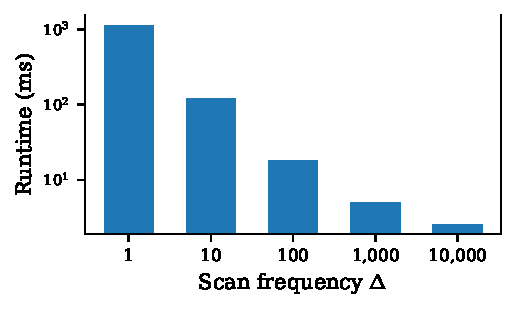
\includegraphics[width=\columnwidth]{fig/ex1_h_vs_time.pdf}
\caption{スキャン頻度 $\Delta$ vs. 処理時間（対数軸）.}
\label{fig:ex1}
\end{figure}

図\ref{fig:ex1}に示す通り、$\Delta$ を10倍にするごとに処理時間は概ね10分の1となり、
スキャン回数の削減が直接的に処理コストを削減することが確認された。

%-----------------------------------------------------------------------
\subsection{EX-2: スケーラビリティ}\label{sec:ex2}
%-----------------------------------------------------------------------

ストリーム長 $T$ およびアイテム数 $|\mathcal{I}|$ を独立に変化させ、
処理時間とピークメモリ使用量がどのようにスケールするかを検証する。
$\Delta = T$（バッチ処理）として実行し純計算時間のみを計測した。
合成データ（$\theta = 10$、$W = 120$）に対して $T$・$|\mathcal{I}|$ を独立に変化させた。
基準設定は $T = 10^{5}$、$|\mathcal{I}| = 24$ とし、各軸の変化時は他のパラメータを固定した。

\begin{figure}[t]
\centering
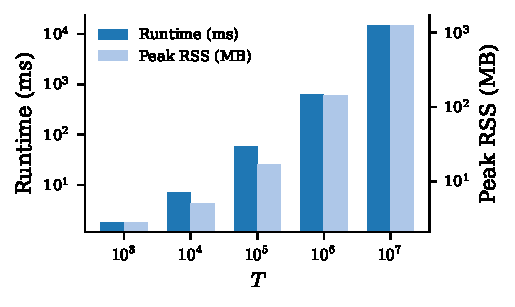
\includegraphics[width=\columnwidth]{fig/ex2_scalability_T.pdf}
\caption{スケーラビリティ vs. $T$：Runtime および Peak RSS.}
\label{fig:ex2t}
\end{figure}

\begin{figure}[t]
\centering
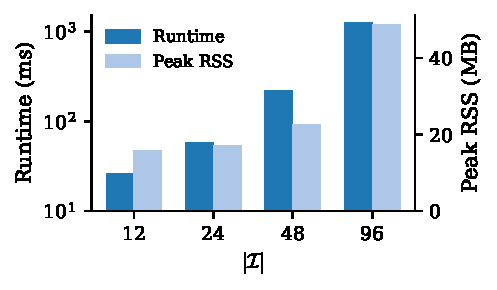
\includegraphics[width=\columnwidth]{fig/ex2_scalability_N.pdf}
\caption{スケーラビリティ vs. $|\mathcal{I}|$：Runtime および Peak RSS.}
\label{fig:ex2n}
\end{figure}

図\ref{fig:ex2t}に示す通り、処理時間は $T$ に対してほぼ線形にスケールし、
$T = 10^{6}$ で 636\,ms、$T = 10^{7}$ で 15{,}108\,ms となった。
図\ref{fig:ex2n}より、$|\mathcal{I}|$ に対しては超線形スケールを示す（$|\mathcal{I}|=96$ で 1{,}272\,ms）が、
これは $|\mathcal{I}|$ 増加により Apriori の高次候補が組み合わせ的に増加するためである。
Peak RSS は $T$ に対してほぼ線形に増加し、$|\mathcal{I}|$ への依存は小さい。

%-----------------------------------------------------------------------
\subsection{EX-3: アブレーション実験}\label{sec:ex3}
%-----------------------------------------------------------------------

Scan Stride Skipping と Apriori Interval Pruning のそれぞれの独立した寄与を定量化し、
両技術を組み合わせることの効果を確認する。
$\Delta = T$（バッチ処理）として実行し純計算時間のみを計測した。
合成データ（$T = 100{,}000$、$|\mathcal{I}| = 48$、$W = 120$、$\theta = 50$、
エポック重複幅 100）に対して下記の4構成の処理時間を計測した。


\begin{figure}[t]
\centering
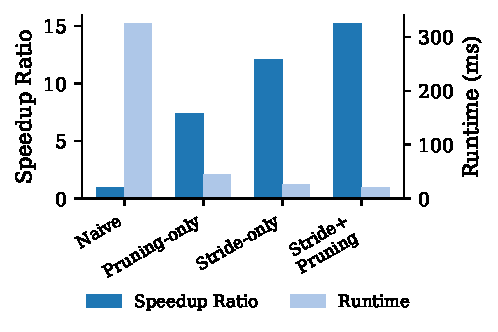
\includegraphics[width=\columnwidth]{fig/ex3_speedup.pdf}
\caption{アブレーション：Naive を基準とした高速化倍率.}
\label{fig:ex3}
\end{figure}

図\ref{fig:ex3}に処理時間および Naive を 1.00 とした高速化倍率を示す。
Full（21.4\,ms）はすべての個別構成を上回る。
Scan Stride Skipping が主要な寄与因子であり、
Naive 比 12.1$\times$ の高速化をもたらす。
Apriori Interval Pruning は単独では 7.4$\times$ の高速化をもたらし、
Stride Skipping と組み合わせることで 15.2$\times$ の高速化を実現する。
2つの技術は独立かつ相補的に寄与することが確認された。

%-----------------------------------------------------------------------
\subsection{EX-4: CASAS センサデータへの適用}\label{sec:ex4}
%-----------------------------------------------------------------------

実センサストリームに提案手法を適用し、
検出された密集区間が解釈可能な行動ルーティンに対応することを確認する。
CASAS スマートホームデータセット~\cite{casas2013} の2系列（hh113・mv001）を使用した。
CASAS は住居内のモーション・接触センサの発火ストリームを記録したものであり、
自律エージェントの行動ログと構造的に類似する。

センサ発火を15分ごとの時間スロットに集約して前処理した（スロット幅 $=$ 15分）。
ウィンドウサイズを $W = 24$スロット（$= 6$時間）に設定し、
1日の特定の時間帯（朝・夕・夜）における行動ルーティンを捕捉できるよう設計した。
スキャン頻度は $\Delta = W = 24$ とした。
各データセットの概要と検出パターン数を表\ref{tab:casas_stats}に示す。

\begin{table}[t]
\caption{CASAS データセット統計.}
\label{tab:casas_stats}
\begin{center}
\begin{tabular}{ccccc}
\hline
データセット & $T$ & $|\mathcal{I}|$ & $\theta$ & パターン数 \\\hline
hh113 & 48{,}901 & 7 & 14 & 26 \\
mv001 & 139{,}033 & 7 & 18 & 34 \\\hline
\end{tabular}
\end{center}
\end{table}

代表的な検出パターンを表\ref{tab:casas_hh113}・表\ref{tab:casas_mv001}に示す。
hh113 では食事関連パターン（DiningRoom+Kitchen：45区間）が卓越し、
キッチン・ダイニングを中心とした日常ルーティンが6時間ウィンドウ内で
繰り返し形成されていることを示す。
mv001 では就寝前の遷移パターン（Bedroom+LivingRoom：113区間）が最頻であり、
リビング滞在 $\to$ 調理 $\to$ 就寝という行動シーケンスが日課として定着していることが示唆される。
いずれのデータセットでも $k \geq 3$ の多アイテムパターンが自動列挙され、
二者間共起では捉えられない複合的な行動遷移が可視化された。

\begin{table}[t]
\caption{hh113における代表的な検出パターン}
\label{tab:casas_hh113}
\begin{center}
\footnotesize
\begin{tabular}{p{3.5cm}cp{2.0cm}}
\hline
センサ組合せ & 区間数 & 推定行動 \\\hline
DiningRoom + Kitchen              & 45 & 食事準備・食事行動 \\
Bathroom + Bedroom                &  8 & 起床・就寝ルーティン \\
DiningRoom + Kitchen + OutsideDoor &  7 & 外出前後の食事行動 \\\hline
\end{tabular}
\end{center}
\end{table}

\begin{table}[t]
\caption{mv001における代表的な検出パターン}
\label{tab:casas_mv001}
\begin{center}
\footnotesize
\begin{tabular}{p{3.5cm}cp{2.0cm}}
\hline
センサ組合せ & 区間数 & 推定行動 \\\hline
Bedroom + LivingRoom          & 113 & 就寝前リビング→寝室 \\
Kitchen + LivingRoom          &  66 & 調理後リビング滞在 \\
Bedroom + Kitchen             &  44 & 就寝前・起床直後 \\
Bedroom + Kitchen + LivingRoom &  44 & 夕方〜就寝前連鎖 \\\hline
\end{tabular}
\end{center}
\end{table}
